The convolutional neural networks are the feed-forwards neural 
networks which contains alternative convolutional layers and sampling 
layer which at the end is connected to fully connected neural networks \citep{liew2016gender}.
The objective of the convolutional layers is to extract the features from 
the given input image samples by applying filters which is used in the training 
of overall network.

\begin{figure}[!htp]
    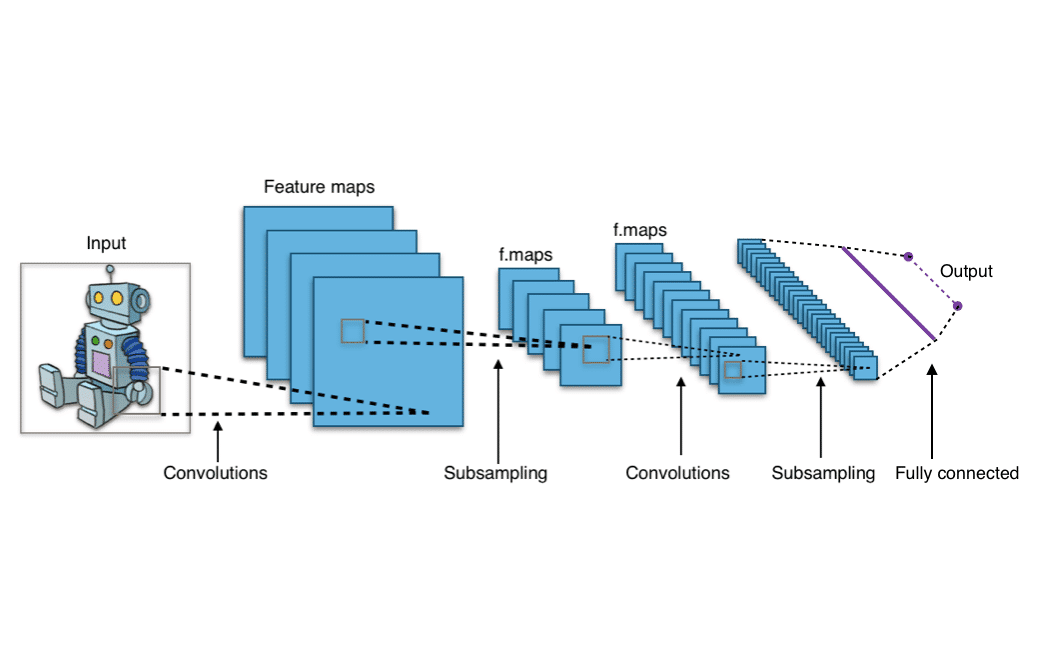
\includegraphics[width=\textwidth]{Images/cnn.png}
    \caption{Convolutional Neural Network}
    \label{figure:cnnf}
\end{figure}
The initial layer is known as the input layer in convolutional network 
which contains the pixel information of the image. The convolutional layer 
of the network determines the output of the neuron of perticular region 
by applying image kernels to extract the features from the images \citep{DBLP:journals/corr/OSheaN15}. 
The image kernels are the matrix of filter which are computed with the local region 
and produce the feature maps  \citep{DBLP:journals/corr/OSheaN15}. 
Furthermore as shown in \ref{figure:cnnf} sub sampling also 
known as downsampling is applied to the feature maps to reduce the dimensionality 
of the feature maps. In addition, there can exist various number of 
convolutional layers and sub sampling layer based on the architecture of the network.
The next layer in the network is flattening layer which reshapes the 
feature maps extract from previous convolutional layers of the network. 
At last the flattened information is passed to the fully connected neural network to analyse the relationships 
in the data and make appropriate predictions \citep{DBLP:journals/corr/OSheaN15}.  
\pagebreak